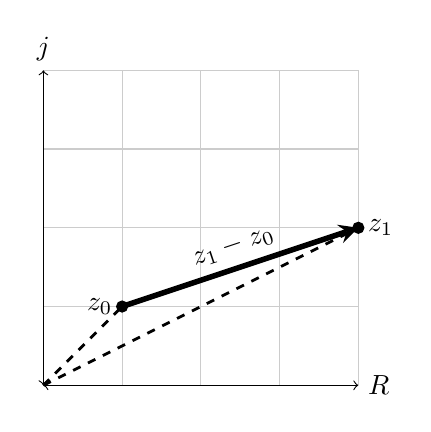
\begin{tikzpicture}
    \draw [thin,gray!40] (0,0) grid (4,4);
    \draw[<->] (0,0)--(4,0) node[right] {$R$};
    \draw[<->] (0,0)--(0,4) node[above]{$j$};
    \coordinate (a) at (1,1);
    \coordinate (b) at (4,2);
    \draw[fill=black] (a) circle(2pt) node[left]{$z_0$};
    \draw[fill=black] (b) circle(2pt) node[right]{$z_1$};
    \draw[line width=2pt,black,-stealth] (a)--(b) node[midway, above, sloped]{$z_1-z_0$};
    \draw[line width=1pt,black,dashed] (0,0)--(a);
    \draw[line width=1pt,black,dashed] (0,0)--(b);
\end{tikzpicture}